\documentclass[twoside]{book}

% Packages required by doxygen
\usepackage{fixltx2e}
\usepackage{calc}
\usepackage{doxygen}
\usepackage[export]{adjustbox} % also loads graphicx
\usepackage{graphicx}
\usepackage[utf8]{inputenc}
\usepackage{makeidx}
\usepackage{multicol}
\usepackage{multirow}
\PassOptionsToPackage{warn}{textcomp}
\usepackage{textcomp}
\usepackage[nointegrals]{wasysym}
\usepackage[table]{xcolor}

% Font selection
\usepackage[T1]{fontenc}
\usepackage[scaled=.90]{helvet}
\usepackage{courier}
\usepackage{amssymb}
\usepackage{sectsty}
\renewcommand{\familydefault}{\sfdefault}
\allsectionsfont{%
  \fontseries{bc}\selectfont%
  \color{darkgray}%
}
\renewcommand{\DoxyLabelFont}{%
  \fontseries{bc}\selectfont%
  \color{darkgray}%
}
\newcommand{\+}{\discretionary{\mbox{\scriptsize$\hookleftarrow$}}{}{}}

% Page & text layout
\usepackage{geometry}
\geometry{%
  a4paper,%
  top=2.5cm,%
  bottom=2.5cm,%
  left=2.5cm,%
  right=2.5cm%
}
\tolerance=750
\hfuzz=15pt
\hbadness=750
\setlength{\emergencystretch}{15pt}
\setlength{\parindent}{0cm}
\setlength{\parskip}{3ex plus 2ex minus 2ex}
\makeatletter
\renewcommand{\paragraph}{%
  \@startsection{paragraph}{4}{0ex}{-1.0ex}{1.0ex}{%
    \normalfont\normalsize\bfseries\SS@parafont%
  }%
}
\renewcommand{\subparagraph}{%
  \@startsection{subparagraph}{5}{0ex}{-1.0ex}{1.0ex}{%
    \normalfont\normalsize\bfseries\SS@subparafont%
  }%
}
\makeatother

% Headers & footers
\usepackage{fancyhdr}
\pagestyle{fancyplain}
\fancyhead[LE]{\fancyplain{}{\bfseries\thepage}}
\fancyhead[CE]{\fancyplain{}{}}
\fancyhead[RE]{\fancyplain{}{\bfseries\leftmark}}
\fancyhead[LO]{\fancyplain{}{\bfseries\rightmark}}
\fancyhead[CO]{\fancyplain{}{}}
\fancyhead[RO]{\fancyplain{}{\bfseries\thepage}}
\fancyfoot[LE]{\fancyplain{}{}}
\fancyfoot[CE]{\fancyplain{}{}}
\fancyfoot[RE]{\fancyplain{}{\bfseries\scriptsize Generated by Doxygen }}
\fancyfoot[LO]{\fancyplain{}{\bfseries\scriptsize Generated by Doxygen }}
\fancyfoot[CO]{\fancyplain{}{}}
\fancyfoot[RO]{\fancyplain{}{}}
\renewcommand{\footrulewidth}{0.4pt}
\renewcommand{\chaptermark}[1]{%
  \markboth{#1}{}%
}
\renewcommand{\sectionmark}[1]{%
  \markright{\thesection\ #1}%
}

% Indices & bibliography
\usepackage{natbib}
\usepackage[titles]{tocloft}
\setcounter{tocdepth}{3}
\setcounter{secnumdepth}{5}
\makeindex

% Hyperlinks (required, but should be loaded last)
\usepackage{ifpdf}
\ifpdf
  \usepackage[pdftex,pagebackref=true]{hyperref}
\else
  \usepackage[ps2pdf,pagebackref=true]{hyperref}
\fi
\hypersetup{%
  colorlinks=true,%
  linkcolor=blue,%
  citecolor=blue,%
  unicode%
}

% Custom commands
\newcommand{\clearemptydoublepage}{%
  \newpage{\pagestyle{empty}\cleardoublepage}%
}

\usepackage{caption}
\captionsetup{labelsep=space,justification=centering,font={bf},singlelinecheck=off,skip=4pt,position=top}

%===== C O N T E N T S =====

\begin{document}

% Titlepage & ToC
\hypersetup{pageanchor=false,
             bookmarksnumbered=true,
             pdfencoding=unicode
            }
\pagenumbering{alph}
\begin{titlepage}
\vspace*{7cm}
\begin{center}%
{\Large Venus \\[1ex]\large 0 }\\
\vspace*{1cm}
{\large Generated by Doxygen 1.8.13}\\
\end{center}
\end{titlepage}
\clearemptydoublepage
\pagenumbering{roman}
\tableofcontents
\clearemptydoublepage
\pagenumbering{arabic}
\hypersetup{pageanchor=true}

%--- Begin generated contents ---
\chapter{Data Structure Index}
\section{Data Structures}
Here are the data structures with brief descriptions\+:\begin{DoxyCompactList}
\item\contentsline{section}{\hyperlink{structvpanel}{vpanel} }{\pageref{structvpanel}}{}
\item\contentsline{section}{\hyperlink{structvtext__field}{vtext\+\_\+field} }{\pageref{structvtext__field}}{}
\item\contentsline{section}{\hyperlink{structvtheme}{vtheme} }{\pageref{structvtheme}}{}
\item\contentsline{section}{\hyperlink{structwidget__t}{widget\+\_\+t} }{\pageref{structwidget__t}}{}
\item\contentsline{section}{\hyperlink{structwindow}{window} \\*Structure that contains the basic building blocks for each venus window }{\pageref{structwindow}}{}
\end{DoxyCompactList}

\chapter{File Index}
\section{File List}
Here is a list of all documented files with brief descriptions\+:\begin{DoxyCompactList}
\item\contentsline{section}{\hyperlink{venus_8h}{venus.\+h} }{\pageref{venus_8h}}{}
\item\contentsline{section}{\hyperlink{venus__common_8h}{venus\+\_\+common.\+h} }{\pageref{venus__common_8h}}{}
\item\contentsline{section}{\hyperlink{window_8c}{window.\+c} }{\pageref{window_8c}}{}
\item\contentsline{section}{\hyperlink{window_8h}{window.\+h} }{\pageref{window_8h}}{}
\item\contentsline{section}{engine/\hyperlink{graphics_8c}{graphics.\+c} }{\pageref{graphics_8c}}{}
\item\contentsline{section}{engine/\hyperlink{graphics_8h}{graphics.\+h} }{\pageref{graphics_8h}}{}
\item\contentsline{section}{toolkit/\hyperlink{default__theme_8c}{default\+\_\+theme.\+c} \\*The default theme for Venus and a good template to design new themes }{\pageref{default__theme_8c}}{}
\item\contentsline{section}{toolkit/\hyperlink{default__theme_8h}{default\+\_\+theme.\+h} \\*Headers for default Venus theme }{\pageref{default__theme_8h}}{}
\item\contentsline{section}{toolkit/\hyperlink{theme_8h}{theme.\+h} \\*Venus theme }{\pageref{theme_8h}}{}
\item\contentsline{section}{toolkit/\hyperlink{widget_8c}{widget.\+c} }{\pageref{widget_8c}}{}
\item\contentsline{section}{toolkit/\hyperlink{widget_8h}{widget.\+h} }{\pageref{widget_8h}}{}
\item\contentsline{section}{toolkit/widgets/\hyperlink{panel_8c}{panel.\+c} }{\pageref{panel_8c}}{}
\item\contentsline{section}{toolkit/widgets/\hyperlink{panel_8h}{panel.\+h} }{\pageref{panel_8h}}{}
\item\contentsline{section}{toolkit/widgets/\hyperlink{text__field_8c}{text\+\_\+field.\+c} }{\pageref{text__field_8c}}{}
\item\contentsline{section}{toolkit/widgets/\hyperlink{text__field_8h}{text\+\_\+field.\+h} }{\pageref{text__field_8h}}{}
\item\contentsline{section}{util/\hyperlink{matrix_8h}{matrix.\+h} }{\pageref{matrix_8h}}{}
\item\contentsline{section}{util/\hyperlink{types_8c}{types.\+c} }{\pageref{types_8c}}{}
\item\contentsline{section}{util/\hyperlink{types_8h}{types.\+h} \\*Includes some basic types Venus Graphics Engine Copyright (C) 2020, Wesley Studt }{\pageref{types_8h}}{}
\item\contentsline{section}{util/\hyperlink{vector_8h}{vector.\+h} }{\pageref{vector_8h}}{}
\end{DoxyCompactList}

\chapter{Data Structure Documentation}
\hypertarget{structmatrix}{}\section{matrix Struct Reference}
\label{structmatrix}\index{matrix@{matrix}}
\subsection*{Data Fields}
\begin{DoxyCompactItemize}
\item 
\mbox{\Hypertarget{structmatrix_ae8233ee9da9814d9c712a855f882d95e}\label{structmatrix_ae8233ee9da9814d9c712a855f882d95e}} 
unsigned {\bfseries rows}
\item 
\mbox{\Hypertarget{structmatrix_ae8349789b2a17e41e61df5a47481b76d}\label{structmatrix_ae8349789b2a17e41e61df5a47481b76d}} 
unsigned {\bfseries columns}
\item 
\mbox{\Hypertarget{structmatrix_a130b05d829c7f46ee353df0c466bbcb1}\label{structmatrix_a130b05d829c7f46ee353df0c466bbcb1}} 
float $\ast$ {\bfseries data}
\end{DoxyCompactItemize}


The documentation for this struct was generated from the following file\+:\begin{DoxyCompactItemize}
\item 
util/\hyperlink{matrix_8h}{matrix.\+h}\end{DoxyCompactItemize}

\hypertarget{structvector}{}\section{vector Struct Reference}
\label{structvector}\index{vector@{vector}}
\subsection*{Data Fields}
\begin{DoxyCompactItemize}
\item 
\mbox{\Hypertarget{structvector_aca6d41fa0791981e3d76e6c2c4da7f5b}\label{structvector_aca6d41fa0791981e3d76e6c2c4da7f5b}} 
unsigned {\bfseries size}
\item 
\mbox{\Hypertarget{structvector_a7425cdf0642c0e45759b4e46772ff1b5}\label{structvector_a7425cdf0642c0e45759b4e46772ff1b5}} 
float $\ast$ {\bfseries data}
\end{DoxyCompactItemize}


The documentation for this struct was generated from the following file\+:\begin{DoxyCompactItemize}
\item 
util/\hyperlink{vector_8h}{vector.\+h}\end{DoxyCompactItemize}

\hypertarget{structwindow}{}\section{window Struct Reference}
\label{structwindow}\index{window@{window}}


Structure that contains the basic building blocks for each venus window.  




{\ttfamily \#include $<$window.\+h$>$}

\subsection*{Data Fields}
\begin{DoxyCompactItemize}
\item 
\mbox{\Hypertarget{structwindow_a6d1d235e4e25a3ffee451f880ff3d936}\label{structwindow_a6d1d235e4e25a3ffee451f880ff3d936}} 
int \hyperlink{structwindow_a6d1d235e4e25a3ffee451f880ff3d936}{width}
\begin{DoxyCompactList}\small\item\em The width of the window. \end{DoxyCompactList}\item 
\mbox{\Hypertarget{structwindow_a3fbcf84b22b22fff0eb213414871aad9}\label{structwindow_a3fbcf84b22b22fff0eb213414871aad9}} 
int \hyperlink{structwindow_a3fbcf84b22b22fff0eb213414871aad9}{height}
\begin{DoxyCompactList}\small\item\em The height of the window. \end{DoxyCompactList}\item 
\mbox{\Hypertarget{structwindow_a90eff798620fee3c37913a2a50f1c2a8}\label{structwindow_a90eff798620fee3c37913a2a50f1c2a8}} 
\+\_\+\+\_\+glx\+\_\+context $\ast$ \hyperlink{structwindow_a90eff798620fee3c37913a2a50f1c2a8}{context}
\begin{DoxyCompactList}\small\item\em Pointer to the window\textquotesingle{}s unique G\+L\+X\+Context. \end{DoxyCompactList}\item 
\mbox{\Hypertarget{structwindow_a23ff6e8e3c92fbe719eac958c837303d}\label{structwindow_a23ff6e8e3c92fbe719eac958c837303d}} 
\+\_\+\+\_\+x\+\_\+win \hyperlink{structwindow_a23ff6e8e3c92fbe719eac958c837303d}{xwin}
\begin{DoxyCompactList}\small\item\em The actual window. \end{DoxyCompactList}\end{DoxyCompactItemize}


\subsection{Detailed Description}
Structure that contains the basic building blocks for each venus window. 

It carries an X Window and a pointer to it\textquotesingle{}s own separate G\+L\+X\+Context that can be used to draw on the window. 

The documentation for this struct was generated from the following file\+:\begin{DoxyCompactItemize}
\item 
\hyperlink{window_8h}{window.\+h}\end{DoxyCompactItemize}

\chapter{File Documentation}
\hypertarget{matrix_8c}{}\section{util/matrix.c File Reference}
\label{matrix_8c}\index{util/matrix.\+c@{util/matrix.\+c}}
{\ttfamily \#include \char`\"{}matrix.\+h\char`\"{}}\newline
{\ttfamily \#include \char`\"{}../venus\+\_\+common.\+h\char`\"{}}\newline
{\ttfamily \#include $<$stdio.\+h$>$}\newline
{\ttfamily \#include $<$stdlib.\+h$>$}\newline
{\ttfamily \#include $<$memory.\+h$>$}\newline
Include dependency graph for matrix.\+c\+:\nopagebreak
\begin{figure}[H]
\begin{center}
\leavevmode
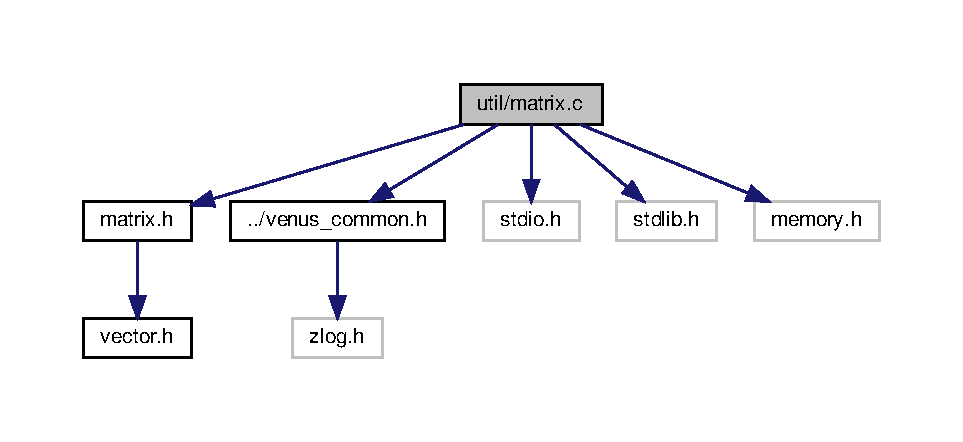
\includegraphics[width=350pt]{matrix_8c__incl}
\end{center}
\end{figure}
\subsection*{Functions}
\begin{DoxyCompactItemize}
\item 
\mbox{\Hypertarget{matrix_8c_aa5051f95897c098f254782851412bed7}\label{matrix_8c_aa5051f95897c098f254782851412bed7}} 
int {\bfseries check\+\_\+matrix\+\_\+size} (\hyperlink{structmatrix}{matrix} $\ast$mat0, \hyperlink{structmatrix}{matrix} $\ast$mat1)
\item 
\mbox{\Hypertarget{matrix_8c_a87b07bd837d135d2b135b80e1e938d58}\label{matrix_8c_a87b07bd837d135d2b135b80e1e938d58}} 
\hyperlink{structmatrix}{matrix} {\bfseries create\+\_\+matrix} (unsigned rows, unsigned columns)
\item 
\mbox{\Hypertarget{matrix_8c_a64f71ab93eed506021b09bc6d2dfe019}\label{matrix_8c_a64f71ab93eed506021b09bc6d2dfe019}} 
void {\bfseries resize\+\_\+matrix} (\hyperlink{structmatrix}{matrix} $\ast$matrix0, unsigned new\+\_\+rows, unsigned new\+\_\+columns)
\item 
\mbox{\Hypertarget{matrix_8c_a2c03755da83185ee7f4203905db3a53d}\label{matrix_8c_a2c03755da83185ee7f4203905db3a53d}} 
int {\bfseries format\+\_\+matrix} (\hyperlink{structmatrix}{matrix} $\ast$mat, \hyperlink{structmatrix}{matrix} $\ast$format)
\item 
\mbox{\Hypertarget{matrix_8c_ad60d2628e1285f8eada6ae607bd4149d}\label{matrix_8c_ad60d2628e1285f8eada6ae607bd4149d}} 
int {\bfseries matrix\+\_\+copy} (\hyperlink{structmatrix}{matrix} $\ast$destination, \hyperlink{structmatrix}{matrix} $\ast$source)
\item 
\mbox{\Hypertarget{matrix_8c_a667c88bd2498eb84d397f1db46c96479}\label{matrix_8c_a667c88bd2498eb84d397f1db46c96479}} 
int {\bfseries matrix\+\_\+negate} (\hyperlink{structmatrix}{matrix} $\ast$destination, \hyperlink{structmatrix}{matrix} $\ast$source)
\item 
\mbox{\Hypertarget{matrix_8c_acfec626349aa6e65c7207bc48f7ea60e}\label{matrix_8c_acfec626349aa6e65c7207bc48f7ea60e}} 
int {\bfseries matrix\+\_\+add} (\hyperlink{structmatrix}{matrix} $\ast$destination, \hyperlink{structmatrix}{matrix} $\ast$source0, \hyperlink{structmatrix}{matrix} $\ast$source1)
\item 
\mbox{\Hypertarget{matrix_8c_a8dbe07e7f678d239299e1acd7ad02894}\label{matrix_8c_a8dbe07e7f678d239299e1acd7ad02894}} 
int {\bfseries matrix\+\_\+subtract} (\hyperlink{structmatrix}{matrix} $\ast$destination, \hyperlink{structmatrix}{matrix} $\ast$source0, \hyperlink{structmatrix}{matrix} $\ast$source1)
\item 
\mbox{\Hypertarget{matrix_8c_adb975525d21611c7a3a7f4e1eb4abb3e}\label{matrix_8c_adb975525d21611c7a3a7f4e1eb4abb3e}} 
int {\bfseries matrix\+\_\+multiply\+\_\+scalar} (\hyperlink{structmatrix}{matrix} $\ast$destination, \hyperlink{structmatrix}{matrix} $\ast$source, float scalar)
\item 
\mbox{\Hypertarget{matrix_8c_a9438c6eb7ff5cfc8b3b63e8deafc9b6f}\label{matrix_8c_a9438c6eb7ff5cfc8b3b63e8deafc9b6f}} 
int {\bfseries matrix\+\_\+transpose} (\hyperlink{structmatrix}{matrix} $\ast$destination, \hyperlink{structmatrix}{matrix} $\ast$source)
\item 
\mbox{\Hypertarget{matrix_8c_a2bb840b7553796e6fcd091d5c7d32c3b}\label{matrix_8c_a2bb840b7553796e6fcd091d5c7d32c3b}} 
void {\bfseries print\+\_\+matrix} (\hyperlink{structmatrix}{matrix} $\ast$mat)
\end{DoxyCompactItemize}

\hypertarget{matrix_8h}{}\section{util/matrix.h File Reference}
\label{matrix_8h}\index{util/matrix.\+h@{util/matrix.\+h}}
{\ttfamily \#include $<$stdlib.\+h$>$}\newline
{\ttfamily \#include $<$string.\+h$>$}\newline
{\ttfamily \#include $<$stdio.\+h$>$}\newline
Include dependency graph for matrix.\+h\+:\nopagebreak
\begin{figure}[H]
\begin{center}
\leavevmode
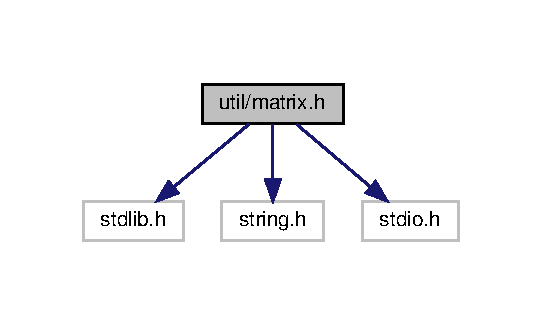
\includegraphics[width=260pt]{matrix_8h__incl}
\end{center}
\end{figure}
\subsection*{Macros}
\begin{DoxyCompactItemize}
\item 
\mbox{\Hypertarget{matrix_8h_a69d543f0ecb517b2913fde69011b5c15}\label{matrix_8h_a69d543f0ecb517b2913fde69011b5c15}} 
\#define {\bfseries V\+S\+\_\+\+M\+A\+T\+R\+I\+X\+\_\+\+R\+OW}~0
\item 
\mbox{\Hypertarget{matrix_8h_a7ac9faf7957b591b5e7d16d100d783a6}\label{matrix_8h_a7ac9faf7957b591b5e7d16d100d783a6}} 
\#define {\bfseries V\+S\+\_\+\+M\+A\+T\+R\+I\+X\+\_\+\+C\+O\+L\+U\+MN}~1
\item 
\mbox{\Hypertarget{matrix_8h_ad1a9a4d466b195421b15d4c1f45e0779}\label{matrix_8h_ad1a9a4d466b195421b15d4c1f45e0779}} 
\#define {\bfseries V\+S\+\_\+\+D\+E\+F\+I\+N\+E\+\_\+\+M\+A\+T\+R\+IX}(T\+Y\+PE,  N\+A\+ME)
\end{DoxyCompactItemize}
\subsection*{Functions}
\begin{DoxyCompactItemize}
\item 
\mbox{\Hypertarget{matrix_8h_a24400a6446d24fb1e6a04cd7b9726ea9}\label{matrix_8h_a24400a6446d24fb1e6a04cd7b9726ea9}} 
unsigned {\bfseries matrix\+\_\+rows} (void $\ast$mat)
\item 
\mbox{\Hypertarget{matrix_8h_af1f29557617a9f2e51293c4f5b94067f}\label{matrix_8h_af1f29557617a9f2e51293c4f5b94067f}} 
unsigned {\bfseries matrix\+\_\+columns} (void $\ast$mat)
\item 
\mbox{\Hypertarget{matrix_8h_a7f6fd93a922a8809082d5611b6343d80}\label{matrix_8h_a7f6fd93a922a8809082d5611b6343d80}} 
unsigned {\bfseries matrix\+\_\+size} (void $\ast$mat)
\item 
\mbox{\Hypertarget{matrix_8h_a8c790c31e7ef37d0990377ef82be2ec0}\label{matrix_8h_a8c790c31e7ef37d0990377ef82be2ec0}} 
void {\bfseries matrix\+\_\+delete} (void $\ast$mat)
\end{DoxyCompactItemize}


\subsection{Detailed Description}
Venus Graphics Engine Copyright (C) 2020, Wesley Studt 
\hypertarget{vector_8c}{}\section{util/vector.c File Reference}
\label{vector_8c}\index{util/vector.\+c@{util/vector.\+c}}
{\ttfamily \#include \char`\"{}vector.\+h\char`\"{}}\newline
{\ttfamily \#include $<$stdlib.\+h$>$}\newline
Include dependency graph for vector.\+c\+:\nopagebreak
\begin{figure}[H]
\begin{center}
\leavevmode
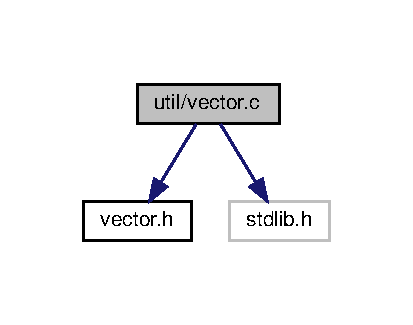
\includegraphics[width=198pt]{vector_8c__incl}
\end{center}
\end{figure}
\subsection*{Functions}
\begin{DoxyCompactItemize}
\item 
\mbox{\Hypertarget{vector_8c_a65592a5df76b614fb217c8ed09e10784}\label{vector_8c_a65592a5df76b614fb217c8ed09e10784}} 
\hyperlink{structvector}{vector} {\bfseries create\+\_\+vector} (unsigned size)
\item 
\mbox{\Hypertarget{vector_8c_a3caa33859c2124565a0e1ee2a4e5006c}\label{vector_8c_a3caa33859c2124565a0e1ee2a4e5006c}} 
float {\bfseries vector\+\_\+dot} (\hyperlink{structvector}{vector} $\ast$vec0, \hyperlink{structvector}{vector} $\ast$vec1)
\item 
\mbox{\Hypertarget{vector_8c_a33de33cda3e7bd8f39bc575db32a3e43}\label{vector_8c_a33de33cda3e7bd8f39bc575db32a3e43}} 
int {\bfseries vector\+\_\+multiply} (\hyperlink{structvector}{vector} $\ast$destination, \hyperlink{structvector}{vector} $\ast$source0, \hyperlink{structvector}{vector} $\ast$source1)
\end{DoxyCompactItemize}

\hypertarget{vector_8h}{}\section{util/vector.h File Reference}
\label{vector_8h}\index{util/vector.\+h@{util/vector.\+h}}
{\ttfamily \#include $<$stdlib.\+h$>$}\newline
{\ttfamily \#include $<$stdarg.\+h$>$}\newline
{\ttfamily \#include $<$string.\+h$>$}\newline
Include dependency graph for vector.\+h\+:\nopagebreak
\begin{figure}[H]
\begin{center}
\leavevmode
\includegraphics[width=196pt]{vector_8h__incl}
\end{center}
\end{figure}
This graph shows which files directly or indirectly include this file\+:\nopagebreak
\begin{figure}[H]
\begin{center}
\leavevmode
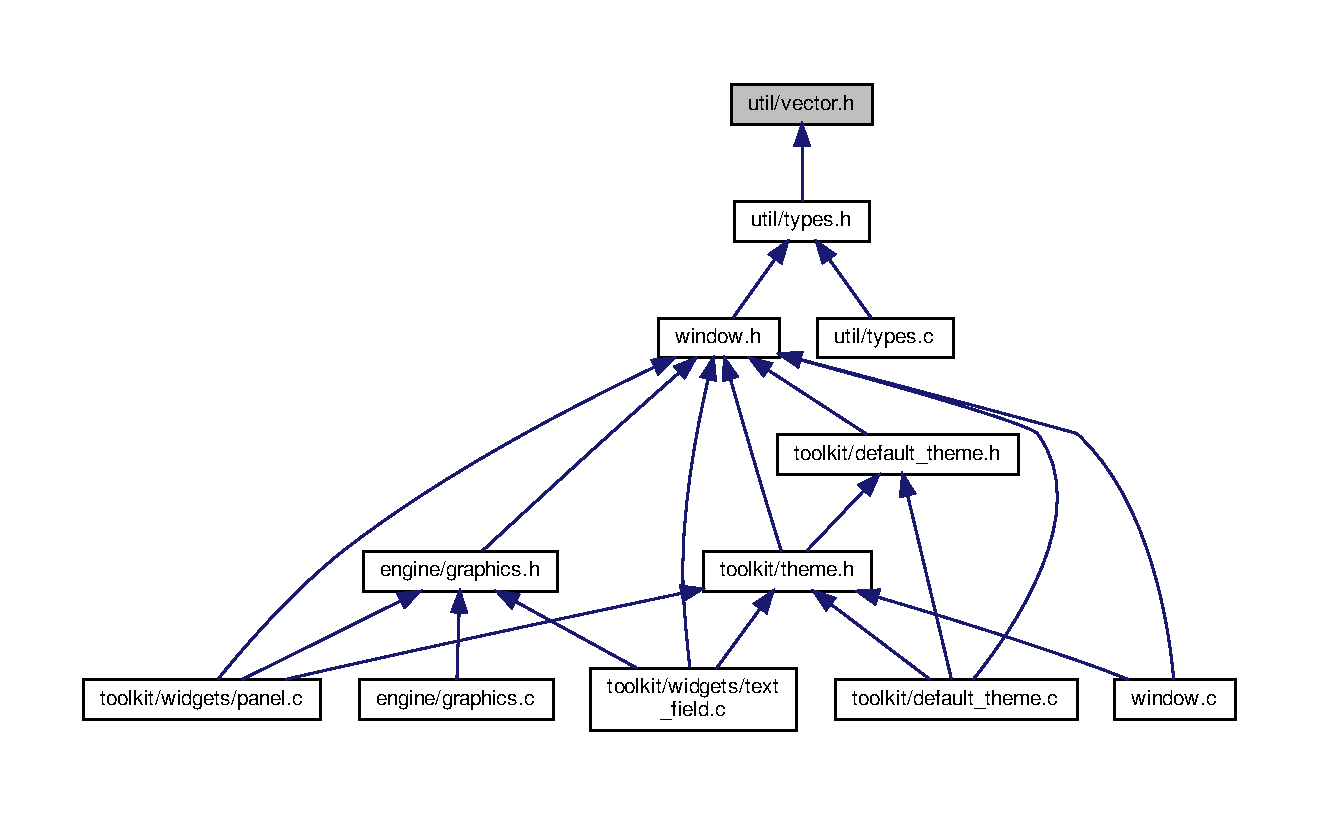
\includegraphics[width=350pt]{vector_8h__dep__incl}
\end{center}
\end{figure}
\subsection*{Macros}
\begin{DoxyCompactItemize}
\item 
\#define \hyperlink{vector_8h_a23408848c6471414c769e5677fe1d21e}{V\+S\+\_\+\+I\+N\+T\+E\+R\+N\+A\+L\+\_\+\+S\+E\+T\+\_\+\+V\+E\+C\+T\+OR}(arg0,  args...)
\begin{DoxyCompactList}\small\item\em Defines a new vector type and includes function prototypes. \end{DoxyCompactList}\item 
\#define {\bfseries V\+S\+\_\+\+D\+E\+F\+I\+N\+E\+\_\+\+V\+E\+C\+T\+O\+R\+\_\+\+H\+E\+A\+D\+ER}(T\+Y\+PE,  N\+A\+ME)
\item 
\#define \hyperlink{vector_8h_a249e54d71982e9aa22445321c9fdd2cd}{V\+S\+\_\+\+D\+E\+F\+I\+N\+E\+\_\+\+V\+E\+C\+T\+O\+R\+\_\+\+S\+O\+U\+R\+CE}(T\+Y\+PE,  N\+A\+ME)
\begin{DoxyCompactList}\small\item\em Provides the source code for a previously defined vector type. \end{DoxyCompactList}\end{DoxyCompactItemize}
\subsection*{Functions}
\begin{DoxyCompactItemize}
\item 
\mbox{\Hypertarget{vector_8h_a6674344a5c5c3672a42e4a10af089846}\label{vector_8h_a6674344a5c5c3672a42e4a10af089846}} 
unsigned {\bfseries vec\+\_\+size} (void $\ast$vec)
\item 
\mbox{\Hypertarget{vector_8h_a94c40f2b664ea6faff87782b8a6826c2}\label{vector_8h_a94c40f2b664ea6faff87782b8a6826c2}} 
void {\bfseries vec\+\_\+delete} (void $\ast$vec)
\end{DoxyCompactItemize}


\subsection{Detailed Description}
Venus Graphics Engine Copyright (C) 2020, Wesley Studt 

\subsection{Macro Definition Documentation}
\mbox{\Hypertarget{vector_8h_aef7794183fb0e54950ce39d24d56e88c}\label{vector_8h_aef7794183fb0e54950ce39d24d56e88c}} 
\index{vector.\+h@{vector.\+h}!V\+S\+\_\+\+D\+E\+F\+I\+N\+E\+\_\+\+V\+E\+C\+T\+O\+R\+\_\+\+H\+E\+A\+D\+ER@{V\+S\+\_\+\+D\+E\+F\+I\+N\+E\+\_\+\+V\+E\+C\+T\+O\+R\+\_\+\+H\+E\+A\+D\+ER}}
\index{V\+S\+\_\+\+D\+E\+F\+I\+N\+E\+\_\+\+V\+E\+C\+T\+O\+R\+\_\+\+H\+E\+A\+D\+ER@{V\+S\+\_\+\+D\+E\+F\+I\+N\+E\+\_\+\+V\+E\+C\+T\+O\+R\+\_\+\+H\+E\+A\+D\+ER}!vector.\+h@{vector.\+h}}
\subsubsection{\texorpdfstring{V\+S\+\_\+\+D\+E\+F\+I\+N\+E\+\_\+\+V\+E\+C\+T\+O\+R\+\_\+\+H\+E\+A\+D\+ER}{VS\_DEFINE\_VECTOR\_HEADER}}
{\footnotesize\ttfamily \#define V\+S\+\_\+\+D\+E\+F\+I\+N\+E\+\_\+\+V\+E\+C\+T\+O\+R\+\_\+\+H\+E\+A\+D\+ER(\begin{DoxyParamCaption}\item[{}]{T\+Y\+PE,  }\item[{}]{N\+A\+ME }\end{DoxyParamCaption})}

{\bfseries Value\+:}
\begin{DoxyCode}
\textcolor{keyword}{typedef} TYPE *NAME;                                                                         \(\backslash\)
                                                                                            \(\backslash\)
NAME create\_##NAME(\textcolor{keywordtype}{unsigned} size);                                                          \(\backslash\)
NAME make\_##NAME(\textcolor{keywordtype}{unsigned} size, ...);                                                       \(\backslash\)
void NAME##\_resize(NAME vec, \textcolor{keywordtype}{unsigned} new\_size);                                            \(\backslash\)
void NAME##\_add(NAME dest, NAME src0, NAME src1);                                           \(\backslash\)
void NAME##\_subtract(NAME dest, NAME src0, NAME src1);                                      \(\backslash\)
void NAME##\_cross(NAME dest, NAME src0, NAME src1);                                         \(\backslash\)
void NAME##\_multiply(NAME dest, NAME src, TYPE scalar);                                     \(\backslash\)
TYPE NAME##\_dot(NAME src0, NAME src1);                                                      \(\backslash\)
\end{DoxyCode}
\mbox{\Hypertarget{vector_8h_a249e54d71982e9aa22445321c9fdd2cd}\label{vector_8h_a249e54d71982e9aa22445321c9fdd2cd}} 
\index{vector.\+h@{vector.\+h}!V\+S\+\_\+\+D\+E\+F\+I\+N\+E\+\_\+\+V\+E\+C\+T\+O\+R\+\_\+\+S\+O\+U\+R\+CE@{V\+S\+\_\+\+D\+E\+F\+I\+N\+E\+\_\+\+V\+E\+C\+T\+O\+R\+\_\+\+S\+O\+U\+R\+CE}}
\index{V\+S\+\_\+\+D\+E\+F\+I\+N\+E\+\_\+\+V\+E\+C\+T\+O\+R\+\_\+\+S\+O\+U\+R\+CE@{V\+S\+\_\+\+D\+E\+F\+I\+N\+E\+\_\+\+V\+E\+C\+T\+O\+R\+\_\+\+S\+O\+U\+R\+CE}!vector.\+h@{vector.\+h}}
\subsubsection{\texorpdfstring{V\+S\+\_\+\+D\+E\+F\+I\+N\+E\+\_\+\+V\+E\+C\+T\+O\+R\+\_\+\+S\+O\+U\+R\+CE}{VS\_DEFINE\_VECTOR\_SOURCE}}
{\footnotesize\ttfamily \#define V\+S\+\_\+\+D\+E\+F\+I\+N\+E\+\_\+\+V\+E\+C\+T\+O\+R\+\_\+\+S\+O\+U\+R\+CE(\begin{DoxyParamCaption}\item[{}]{T\+Y\+PE,  }\item[{}]{N\+A\+ME }\end{DoxyParamCaption})}



Provides the source code for a previously defined vector type. 

The two values need to reflect a vector type defined by V\+S\+\_\+\+D\+E\+F\+I\+N\+E\+\_\+\+V\+E\+C\+T\+O\+R\+\_\+\+H\+E\+A\+D\+ER.


\begin{DoxyParams}{Parameters}
{\em T\+Y\+PE} & The datatype the vector contains \\
\hline
{\em N\+A\+ME} & The name of the vector \\
\hline
\end{DoxyParams}
\mbox{\Hypertarget{vector_8h_a23408848c6471414c769e5677fe1d21e}\label{vector_8h_a23408848c6471414c769e5677fe1d21e}} 
\index{vector.\+h@{vector.\+h}!V\+S\+\_\+\+I\+N\+T\+E\+R\+N\+A\+L\+\_\+\+S\+E\+T\+\_\+\+V\+E\+C\+T\+OR@{V\+S\+\_\+\+I\+N\+T\+E\+R\+N\+A\+L\+\_\+\+S\+E\+T\+\_\+\+V\+E\+C\+T\+OR}}
\index{V\+S\+\_\+\+I\+N\+T\+E\+R\+N\+A\+L\+\_\+\+S\+E\+T\+\_\+\+V\+E\+C\+T\+OR@{V\+S\+\_\+\+I\+N\+T\+E\+R\+N\+A\+L\+\_\+\+S\+E\+T\+\_\+\+V\+E\+C\+T\+OR}!vector.\+h@{vector.\+h}}
\subsubsection{\texorpdfstring{V\+S\+\_\+\+I\+N\+T\+E\+R\+N\+A\+L\+\_\+\+S\+E\+T\+\_\+\+V\+E\+C\+T\+OR}{VS\_INTERNAL\_SET\_VECTOR}}
{\footnotesize\ttfamily \#define V\+S\+\_\+\+I\+N\+T\+E\+R\+N\+A\+L\+\_\+\+S\+E\+T\+\_\+\+V\+E\+C\+T\+OR(\begin{DoxyParamCaption}\item[{}]{arg0,  }\item[{}]{args... }\end{DoxyParamCaption})}



Defines a new vector type and includes function prototypes. 

In Venus, a vector represents a mathematical vector, not a container like std\+::vector. The reason for this is that since Venus is a G\+U\+I/graphics library, it needs to manipulate points in two-\/dimensional space and three-\/dimensional space. This requires functions that can add, multiply, etc., vectors.


\begin{DoxyParams}{Parameters}
{\em T\+Y\+PE} & The datatype the vector should contain \\
\hline
{\em N\+A\+ME} & The name of the new vector \\
\hline
\end{DoxyParams}

\hypertarget{venus_8h}{}\section{venus.\+h File Reference}
\label{venus_8h}\index{venus.\+h@{venus.\+h}}


The main interface to Venus.  


This graph shows which files directly or indirectly include this file\+:\nopagebreak
\begin{figure}[H]
\begin{center}
\leavevmode
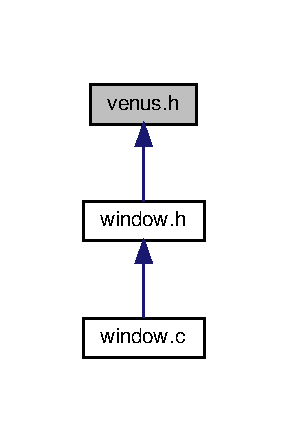
\includegraphics[width=350pt]{venus_8h__dep__incl}
\end{center}
\end{figure}


\subsection{Detailed Description}
The main interface to Venus. 

Venus Graphics Engine Copyright (C) 2020, Wesley Studt 
\hypertarget{venus__common_8h}{}\section{venus\+\_\+common.\+h File Reference}
\label{venus__common_8h}\index{venus\+\_\+common.\+h@{venus\+\_\+common.\+h}}
{\ttfamily \#include $<$zlog.\+h$>$}\newline
Include dependency graph for venus\+\_\+common.\+h\+:\nopagebreak
\begin{figure}[H]
\begin{center}
\leavevmode
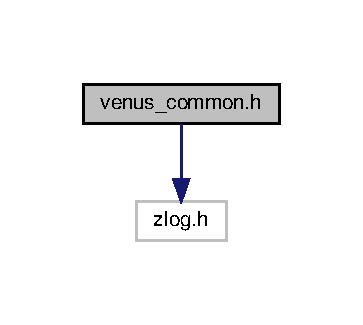
\includegraphics[width=174pt]{venus__common_8h__incl}
\end{center}
\end{figure}
This graph shows which files directly or indirectly include this file\+:\nopagebreak
\begin{figure}[H]
\begin{center}
\leavevmode
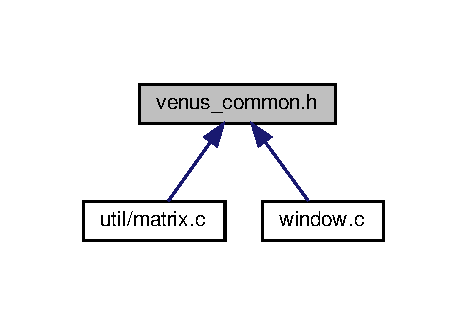
\includegraphics[width=350pt]{venus__common_8h__dep__incl}
\end{center}
\end{figure}
\subsection*{Macros}
\begin{DoxyCompactItemize}
\item 
\mbox{\Hypertarget{venus__common_8h_aa022f8f5073133cb4c385e2fc0c3e613}\label{venus__common_8h_aa022f8f5073133cb4c385e2fc0c3e613}} 
\#define {\bfseries V\+S\+\_\+\+V\+E\+N\+U\+S\+\_\+\+C\+O\+M\+M\+O\+N\+\_\+H}
\item 
\mbox{\Hypertarget{venus__common_8h_ad58799c0c5d62582a981f98ac897973c}\label{venus__common_8h_ad58799c0c5d62582a981f98ac897973c}} 
\#define {\bfseries V\+S\+\_\+\+F\+A\+L\+SE}~0
\item 
\mbox{\Hypertarget{venus__common_8h_a708711345054c692bc1346bcb060c96b}\label{venus__common_8h_a708711345054c692bc1346bcb060c96b}} 
\#define {\bfseries V\+S\+\_\+\+T\+R\+UE}~1
\item 
\mbox{\Hypertarget{venus__common_8h_a940ab0db9205f4237326a7b15b3d7ed1}\label{venus__common_8h_a940ab0db9205f4237326a7b15b3d7ed1}} 
\#define {\bfseries V\+S\+\_\+\+S\+U\+C\+C\+E\+SS}~0x0001
\item 
\mbox{\Hypertarget{venus__common_8h_ab4f37fb879d6c26e7c44d5a1f291b91e}\label{venus__common_8h_ab4f37fb879d6c26e7c44d5a1f291b91e}} 
\#define {\bfseries V\+S\+\_\+\+F\+A\+I\+L\+U\+RE}~0x0000
\item 
\mbox{\Hypertarget{venus__common_8h_a1fc9cc7e10103de2f20b46a7a2c3be61}\label{venus__common_8h_a1fc9cc7e10103de2f20b46a7a2c3be61}} 
\#define {\bfseries V\+S\+\_\+\+F\+A\+I\+L\+\_\+\+V\+E\+N\+US}~0b0010000000000000000000000000000
\item 
\mbox{\Hypertarget{venus__common_8h_a02d4af33f1ac6282ec5d915214f6dd45}\label{venus__common_8h_a02d4af33f1ac6282ec5d915214f6dd45}} 
\#define {\bfseries V\+S\+\_\+\+F\+A\+I\+L\+\_\+\+V\+E\+N\+U\+S\+\_\+\+M\+A\+T\+R\+I\+X\+\_\+\+S\+I\+ZE}~(0x0001 $\vert$ V\+S\+\_\+\+F\+A\+I\+L\+\_\+\+V\+E\+N\+U\+S)
\item 
\mbox{\Hypertarget{venus__common_8h_af14a9bb91f471419c3607d0026b9bd0e}\label{venus__common_8h_af14a9bb91f471419c3607d0026b9bd0e}} 
\#define {\bfseries V\+S\+\_\+\+F\+A\+I\+L\+\_\+\+Z\+L\+OG}~0b0100000000000000000000000000000
\item 
\mbox{\Hypertarget{venus__common_8h_a4d240f1dfa2d1a018d8d93957816e76f}\label{venus__common_8h_a4d240f1dfa2d1a018d8d93957816e76f}} 
\#define {\bfseries V\+S\+\_\+\+F\+A\+I\+L\+\_\+\+Z\+L\+O\+G\+\_\+\+N\+O\+T\+\_\+\+L\+O\+A\+D\+ED}~(0x0001 $\vert$ V\+S\+\_\+\+F\+A\+I\+L\+\_\+\+Z\+L\+O\+G)
\item 
\mbox{\Hypertarget{venus__common_8h_a6f66a858881de221f9083a22892d9611}\label{venus__common_8h_a6f66a858881de221f9083a22892d9611}} 
\#define {\bfseries V\+S\+\_\+\+F\+A\+I\+L\+\_\+\+Z\+L\+O\+G\+\_\+\+M\+I\+S\+S\+I\+N\+G\+\_\+\+C\+A\+T\+E\+G\+O\+RY}~(0x0002 $\vert$ V\+S\+\_\+\+F\+A\+I\+L\+\_\+\+Z\+L\+O\+G)
\item 
\mbox{\Hypertarget{venus__common_8h_a4292a6025bd094ed6ce5e5faeef55287}\label{venus__common_8h_a4292a6025bd094ed6ce5e5faeef55287}} 
\#define {\bfseries V\+S\+\_\+\+F\+A\+I\+L\+\_\+X}~0b1000000000000000000000000000000
\item 
\mbox{\Hypertarget{venus__common_8h_aa71ddf8e707b44753f55fdfc27486147}\label{venus__common_8h_aa71ddf8e707b44753f55fdfc27486147}} 
\#define {\bfseries V\+S\+\_\+\+F\+A\+I\+L\+\_\+\+X\+\_\+\+N\+O\+\_\+\+C\+O\+N\+N\+E\+C\+T\+I\+ON}~(0x0001 $\vert$ V\+S\+\_\+\+F\+A\+I\+L\+\_\+\+X)
\item 
\mbox{\Hypertarget{venus__common_8h_a146680ba9a9c08fe88d51ecd852edec9}\label{venus__common_8h_a146680ba9a9c08fe88d51ecd852edec9}} 
\#define {\bfseries V\+S\+\_\+\+F\+A\+I\+L\+\_\+\+GL}~0b0001000000000000000000000000000
\item 
\mbox{\Hypertarget{venus__common_8h_a0d4421d547cc9e489315271b00481bff}\label{venus__common_8h_a0d4421d547cc9e489315271b00481bff}} 
\#define {\bfseries V\+S\+\_\+\+F\+A\+I\+L\+\_\+\+G\+L\+\_\+\+N\+O\+T\+\_\+\+L\+O\+A\+D\+ED}~(0x0001 $\vert$ V\+S\+\_\+\+F\+A\+I\+L\+\_\+\+G\+L)
\item 
\mbox{\Hypertarget{venus__common_8h_a803b091598468e380fe401472ab20e12}\label{venus__common_8h_a803b091598468e380fe401472ab20e12}} 
\#define {\bfseries V\+S\+\_\+\+F\+A\+I\+L\+\_\+\+G\+LX}~0b0000100000000000000000000000000
\item 
\mbox{\Hypertarget{venus__common_8h_a12388ed07f7be2360734c91ba451e2a1}\label{venus__common_8h_a12388ed07f7be2360734c91ba451e2a1}} 
\#define {\bfseries V\+S\+\_\+\+F\+A\+I\+L\+\_\+\+G\+L\+X\+\_\+\+N\+O\+\_\+\+V\+I\+S\+U\+AL}~(0x0001 $\vert$ V\+S\+\_\+\+F\+A\+I\+L\+\_\+\+G\+L\+X)
\item 
\mbox{\Hypertarget{venus__common_8h_a8840c47197d48d77621861f469ce7d3f}\label{venus__common_8h_a8840c47197d48d77621861f469ce7d3f}} 
\#define {\bfseries V\+S\+\_\+\+F\+A\+I\+L\+\_\+\+G\+L\+X\+\_\+\+I\+N\+V\+A\+L\+I\+D\+\_\+\+V\+E\+R\+S\+I\+ON}~(0x0002 $\vert$ V\+S\+\_\+\+F\+A\+I\+L\+\_\+\+G\+L\+X)
\item 
\mbox{\Hypertarget{venus__common_8h_a1a56a31cd8a771be13afca39e4aa5bc6}\label{venus__common_8h_a1a56a31cd8a771be13afca39e4aa5bc6}} 
\#define {\bfseries vs\+\_\+err}(E\+RR)~\{zlog\+\_\+error(g\+\_\+log, \#E\+RR); return E\+RR;\}
\item 
\mbox{\Hypertarget{venus__common_8h_a32cd33a594289f6294cc132632e38772}\label{venus__common_8h_a32cd33a594289f6294cc132632e38772}} 
\#define {\bfseries vs\+\_\+has\+\_\+err}(X)~!(X)
\end{DoxyCompactItemize}
\subsection*{Variables}
\begin{DoxyCompactItemize}
\item 
\mbox{\Hypertarget{venus__common_8h_a71fea5df2d52de4b3c2e2ad8b18c115c}\label{venus__common_8h_a71fea5df2d52de4b3c2e2ad8b18c115c}} 
zlog\+\_\+category\+\_\+t $\ast$ {\bfseries g\+\_\+log}
\item 
\mbox{\Hypertarget{venus__common_8h_add3ac508f74eb586d528f1346d466bc9}\label{venus__common_8h_add3ac508f74eb586d528f1346d466bc9}} 
int($\ast$ {\bfseries g\+\_\+error\+\_\+callback} )(void $\ast$win, unsigned err)
\end{DoxyCompactItemize}


\subsection{Detailed Description}
Venus Graphics Engine Copyright (C) 2020, Wesley Studt 
\hypertarget{window_8c}{}\section{window.\+c File Reference}
\label{window_8c}\index{window.\+c@{window.\+c}}
{\ttfamily \#include \char`\"{}window.\+h\char`\"{}}\newline
{\ttfamily \#include $<$glad/glad.\+h$>$}\newline
{\ttfamily \#include $<$X11/\+Xlib.\+h$>$}\newline
{\ttfamily \#include $<$X11/\+Xutil.\+h$>$}\newline
{\ttfamily \#include $<$G\+L/glx.\+h$>$}\newline
{\ttfamily \#include $<$stdlib.\+h$>$}\newline
{\ttfamily \#include \char`\"{}venus\+\_\+common.\+h\char`\"{}}\newline
{\ttfamily \#include \char`\"{}toolkit/theme.\+h\char`\"{}}\newline
Include dependency graph for window.\+c\+:\nopagebreak
\begin{figure}[H]
\begin{center}
\leavevmode
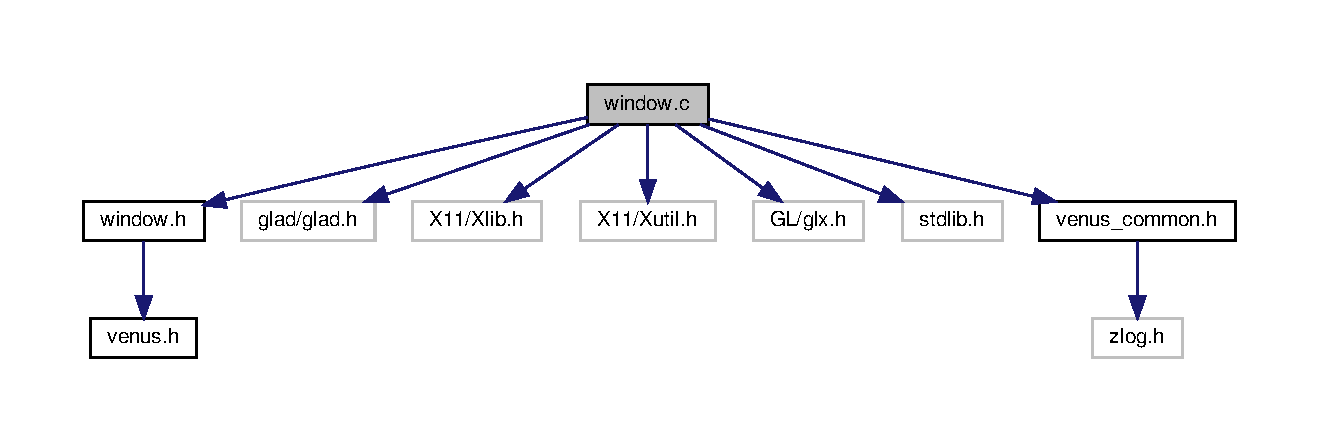
\includegraphics[width=350pt]{window_8c__incl}
\end{center}
\end{figure}
\subsection*{Macros}
\begin{DoxyCompactItemize}
\item 
\mbox{\Hypertarget{window_8c_ac44e7b00d5bc2af9f87b752093e96fcd}\label{window_8c_ac44e7b00d5bc2af9f87b752093e96fcd}} 
\#define {\bfseries G\+L\+X\+\_\+\+C\+O\+N\+T\+E\+X\+T\+\_\+\+M\+A\+J\+O\+R\+\_\+\+V\+E\+R\+S\+I\+O\+N\+\_\+\+A\+RB}~0x2091
\item 
\mbox{\Hypertarget{window_8c_a60923ecde3d05e9be4ec4688af4a186c}\label{window_8c_a60923ecde3d05e9be4ec4688af4a186c}} 
\#define {\bfseries G\+L\+X\+\_\+\+C\+O\+N\+T\+E\+X\+T\+\_\+\+M\+I\+N\+O\+R\+\_\+\+V\+E\+R\+S\+I\+O\+N\+\_\+\+A\+RB}~0x2092
\end{DoxyCompactItemize}
\subsection*{Functions}
\begin{DoxyCompactItemize}
\item 
\mbox{\Hypertarget{window_8c_a1c94ea700a7d193ee3205fbb23e46e23}\label{window_8c_a1c94ea700a7d193ee3205fbb23e46e23}} 
int {\bfseries glx\+\_\+check\+\_\+support} (const char $\ast$ext\+\_\+list, const char $\ast$extension)
\item 
\mbox{\Hypertarget{window_8c_ab40b19047a9a2c12c380c53787fec6f1}\label{window_8c_ab40b19047a9a2c12c380c53787fec6f1}} 
X\+Visual\+Info $\ast$ {\bfseries glx\+\_\+get\+\_\+visual} (int $\ast$attributes, G\+L\+X\+F\+B\+Config $\ast$framebuffer)
\item 
\mbox{\Hypertarget{window_8c_a62c30c52b94a5b224b99eebcf10b3982}\label{window_8c_a62c30c52b94a5b224b99eebcf10b3982}} 
int {\bfseries glx\+\_\+context\+\_\+error} (Display $\ast$display, X\+Error\+Event $\ast$event)
\item 
\mbox{\Hypertarget{window_8c_a3d9562af2832a1fc390c04428fabc326}\label{window_8c_a3d9562af2832a1fc390c04428fabc326}} 
G\+L\+X\+Context {\bfseries glx\+\_\+make\+\_\+context} (X\+Visual\+Info $\ast$visual\+\_\+info, G\+L\+X\+F\+B\+Config framebuffer, G\+L\+X\+Context sharelist, int direct)
\item 
\mbox{\Hypertarget{window_8c_a8210ae1e8beaeb29b2b59ed9f11bf922}\label{window_8c_a8210ae1e8beaeb29b2b59ed9f11bf922}} 
G\+L\+X\+Context {\bfseries make\+\_\+current} (\hyperlink{structwindow}{window} $\ast$\hyperlink{structwindow}{window})
\item 
int \hyperlink{window_8c_affebef5e6a51b1546cadf37adf74297a}{venus\+\_\+initialize} ()
\begin{DoxyCompactList}\small\item\em Initializes venus and the libraries used. \end{DoxyCompactList}\item 
int \hyperlink{window_8c_aa1667db02fb07f04dfb4b96ddec6893d}{create\+\_\+window} (\hyperlink{structwindow}{window} $\ast$win)
\begin{DoxyCompactList}\small\item\em Creates a new window. \end{DoxyCompactList}\item 
int \hyperlink{window_8c_aa2ee2c8b10e2e4536bb4151990f48ac2}{destroy\+\_\+window} (\hyperlink{structwindow}{window} $\ast$win)
\begin{DoxyCompactList}\small\item\em Destroys a window. \end{DoxyCompactList}\item 
int \hyperlink{window_8c_a7ddd3c1fff91f413837be14742e82c5e}{venus\+\_\+terminate} ()
\begin{DoxyCompactList}\small\item\em Terminates venus and does memory clean up. \end{DoxyCompactList}\item 
int \hyperlink{window_8c_a7d2e831da7d3e6cfd60ff95835f1c9fa}{swap\+\_\+buffers} (\hyperlink{structwindow}{window} $\ast$win)
\begin{DoxyCompactList}\small\item\em Swaps the framebuffers and clears the draw buffer. \end{DoxyCompactList}\item 
int \hyperlink{window_8c_aba54f1b4e0762bd4cc0434d4f17a87c4}{set\+\_\+title} (\hyperlink{structwindow}{window} $\ast$win, char $\ast$title)
\begin{DoxyCompactList}\small\item\em Sets a window\textquotesingle{}s title. \end{DoxyCompactList}\item 
int \hyperlink{window_8c_a25032ce093a2111eef67bdebeb5f887c}{set\+\_\+background\+\_\+color} (\hyperlink{structwindow}{window} $\ast$win, color color)
\begin{DoxyCompactList}\small\item\em Sets a window\textquotesingle{}s color. \end{DoxyCompactList}\item 
int \hyperlink{window_8c_a294b947aff88bc133591bc02f3269d51}{show} (\hyperlink{structwindow}{window} $\ast$win)
\begin{DoxyCompactList}\small\item\em Shows a window. \end{DoxyCompactList}\item 
int \hyperlink{window_8c_a1739057d6d8077a7490b0467ea5d064b}{hide} (\hyperlink{structwindow}{window} $\ast$win)
\begin{DoxyCompactList}\small\item\em Hides a window. \end{DoxyCompactList}\item 
int \hyperlink{window_8c_a6a97127a0760a0ca431456fd3fd5c087}{flush} ()
\begin{DoxyCompactList}\small\item\em Flushes all X requests. \end{DoxyCompactList}\item 
int \hyperlink{window_8c_a43891902ce142858e0ee68ce4dff0231}{venus\+\_\+begin\+\_\+loop} ()
\begin{DoxyCompactList}\small\item\em Starts the event loop for any associated venus windows. \end{DoxyCompactList}\end{DoxyCompactItemize}
\subsection*{Variables}
\begin{DoxyCompactItemize}
\item 
\mbox{\Hypertarget{window_8c_aa1d2af63e7bb3256415d7d1ca446fb3b}\label{window_8c_aa1d2af63e7bb3256415d7d1ca446fb3b}} 
Display $\ast$ {\bfseries g\+\_\+display} = N\+U\+LL
\item 
\mbox{\Hypertarget{window_8c_a84b65737d004b98f2d4a95625eff710f}\label{window_8c_a84b65737d004b98f2d4a95625eff710f}} 
Window {\bfseries g\+\_\+root} = 0
\item 
\mbox{\Hypertarget{window_8c_a71fea5df2d52de4b3c2e2ad8b18c115c}\label{window_8c_a71fea5df2d52de4b3c2e2ad8b18c115c}} 
zlog\+\_\+category\+\_\+t $\ast$ {\bfseries g\+\_\+log} = N\+U\+LL
\item 
\mbox{\Hypertarget{window_8c_add3ac508f74eb586d528f1346d466bc9}\label{window_8c_add3ac508f74eb586d528f1346d466bc9}} 
int($\ast$ {\bfseries g\+\_\+error\+\_\+callback} )(void $\ast$win, unsigned err)
\item 
\mbox{\Hypertarget{window_8c_a205f13063e2d37ce36eccb13e03d20e9}\label{window_8c_a205f13063e2d37ce36eccb13e03d20e9}} 
\hyperlink{structwindow}{window} $\ast$ {\bfseries g\+\_\+current\+\_\+window}
\item 
\mbox{\Hypertarget{window_8c_a4cb18135a86a9bb7eea82391beacdbb0}\label{window_8c_a4cb18135a86a9bb7eea82391beacdbb0}} 
int {\bfseries g\+\_\+context\+\_\+err} = 0
\end{DoxyCompactItemize}


\subsection{Detailed Description}
Venus Graphics Engine Copyright (C) 2020, Wesley Studt 

\subsection{Function Documentation}
\mbox{\Hypertarget{window_8c_aa1667db02fb07f04dfb4b96ddec6893d}\label{window_8c_aa1667db02fb07f04dfb4b96ddec6893d}} 
\index{window.\+c@{window.\+c}!create\+\_\+window@{create\+\_\+window}}
\index{create\+\_\+window@{create\+\_\+window}!window.\+c@{window.\+c}}
\subsubsection{\texorpdfstring{create\+\_\+window()}{create\_window()}}
{\footnotesize\ttfamily int create\+\_\+window (\begin{DoxyParamCaption}\item[{\hyperlink{structwindow}{window} $\ast$}]{win }\end{DoxyParamCaption})}



Creates a new window. 

This creates a new X window and binds a GL context to that window.


\begin{DoxyParams}{Parameters}
{\em win} & Pointer to window\\
\hline
\end{DoxyParams}
\begin{DoxyReturn}{Returns}
Returns whether it was successful or not 
\end{DoxyReturn}
\mbox{\Hypertarget{window_8c_aa2ee2c8b10e2e4536bb4151990f48ac2}\label{window_8c_aa2ee2c8b10e2e4536bb4151990f48ac2}} 
\index{window.\+c@{window.\+c}!destroy\+\_\+window@{destroy\+\_\+window}}
\index{destroy\+\_\+window@{destroy\+\_\+window}!window.\+c@{window.\+c}}
\subsubsection{\texorpdfstring{destroy\+\_\+window()}{destroy\_window()}}
{\footnotesize\ttfamily int destroy\+\_\+window (\begin{DoxyParamCaption}\item[{\hyperlink{structwindow}{window} $\ast$}]{win }\end{DoxyParamCaption})}



Destroys a window. 

You should always destroy any window you create in order to ensure that no memory is leaked.


\begin{DoxyParams}{Parameters}
{\em win} & Pointer to window\\
\hline
\end{DoxyParams}
Returns whether it was successful or not \mbox{\Hypertarget{window_8c_a6a97127a0760a0ca431456fd3fd5c087}\label{window_8c_a6a97127a0760a0ca431456fd3fd5c087}} 
\index{window.\+c@{window.\+c}!flush@{flush}}
\index{flush@{flush}!window.\+c@{window.\+c}}
\subsubsection{\texorpdfstring{flush()}{flush()}}
{\footnotesize\ttfamily int flush (\begin{DoxyParamCaption}{ }\end{DoxyParamCaption})}



Flushes all X requests. 

This is only used to tell X to flush the display. It will likely be removed soon because it won\textquotesingle{}t need to exist.

\begin{DoxyReturn}{Returns}
Returns whether it was successful or not 
\end{DoxyReturn}
\mbox{\Hypertarget{window_8c_a1739057d6d8077a7490b0467ea5d064b}\label{window_8c_a1739057d6d8077a7490b0467ea5d064b}} 
\index{window.\+c@{window.\+c}!hide@{hide}}
\index{hide@{hide}!window.\+c@{window.\+c}}
\subsubsection{\texorpdfstring{hide()}{hide()}}
{\footnotesize\ttfamily int hide (\begin{DoxyParamCaption}\item[{\hyperlink{structwindow}{window} $\ast$}]{win }\end{DoxyParamCaption})}



Hides a window. 

This requests X to unmap the window


\begin{DoxyParams}{Parameters}
{\em win} & Pointer to window\\
\hline
\end{DoxyParams}
\begin{DoxyReturn}{Returns}
Returns whether it was successful or not 
\end{DoxyReturn}
\mbox{\Hypertarget{window_8c_a25032ce093a2111eef67bdebeb5f887c}\label{window_8c_a25032ce093a2111eef67bdebeb5f887c}} 
\index{window.\+c@{window.\+c}!set\+\_\+background\+\_\+color@{set\+\_\+background\+\_\+color}}
\index{set\+\_\+background\+\_\+color@{set\+\_\+background\+\_\+color}!window.\+c@{window.\+c}}
\subsubsection{\texorpdfstring{set\+\_\+background\+\_\+color()}{set\_background\_color()}}
{\footnotesize\ttfamily int set\+\_\+background\+\_\+color (\begin{DoxyParamCaption}\item[{\hyperlink{structwindow}{window} $\ast$}]{win,  }\item[{color}]{color }\end{DoxyParamCaption})}



Sets a window\textquotesingle{}s color. 


\begin{DoxyParams}{Parameters}
{\em win} & Pointer to window \\
\hline
{\em color} & The window\textquotesingle{}s color. Only the first three values, the red, green, and blue values, are used.\\
\hline
\end{DoxyParams}
\begin{DoxyReturn}{Returns}
Returns whether it was successful or not 
\end{DoxyReturn}
\mbox{\Hypertarget{window_8c_aba54f1b4e0762bd4cc0434d4f17a87c4}\label{window_8c_aba54f1b4e0762bd4cc0434d4f17a87c4}} 
\index{window.\+c@{window.\+c}!set\+\_\+title@{set\+\_\+title}}
\index{set\+\_\+title@{set\+\_\+title}!window.\+c@{window.\+c}}
\subsubsection{\texorpdfstring{set\+\_\+title()}{set\_title()}}
{\footnotesize\ttfamily int set\+\_\+title (\begin{DoxyParamCaption}\item[{\hyperlink{structwindow}{window} $\ast$}]{win,  }\item[{char $\ast$}]{title }\end{DoxyParamCaption})}



Sets a window\textquotesingle{}s title. 


\begin{DoxyParams}{Parameters}
{\em win} & Pointer to window \\
\hline
{\em title} & The desired title\\
\hline
\end{DoxyParams}
\begin{DoxyReturn}{Returns}
Returns whether it was successful or not 
\end{DoxyReturn}
\mbox{\Hypertarget{window_8c_a294b947aff88bc133591bc02f3269d51}\label{window_8c_a294b947aff88bc133591bc02f3269d51}} 
\index{window.\+c@{window.\+c}!show@{show}}
\index{show@{show}!window.\+c@{window.\+c}}
\subsubsection{\texorpdfstring{show()}{show()}}
{\footnotesize\ttfamily int show (\begin{DoxyParamCaption}\item[{\hyperlink{structwindow}{window} $\ast$}]{win }\end{DoxyParamCaption})}



Shows a window. 

This requests X to map the window


\begin{DoxyParams}{Parameters}
{\em win} & Pointer to window\\
\hline
\end{DoxyParams}
\begin{DoxyReturn}{Returns}
Returns whether it was successful or not 
\end{DoxyReturn}
\mbox{\Hypertarget{window_8c_a7d2e831da7d3e6cfd60ff95835f1c9fa}\label{window_8c_a7d2e831da7d3e6cfd60ff95835f1c9fa}} 
\index{window.\+c@{window.\+c}!swap\+\_\+buffers@{swap\+\_\+buffers}}
\index{swap\+\_\+buffers@{swap\+\_\+buffers}!window.\+c@{window.\+c}}
\subsubsection{\texorpdfstring{swap\+\_\+buffers()}{swap\_buffers()}}
{\footnotesize\ttfamily int swap\+\_\+buffers (\begin{DoxyParamCaption}\item[{\hyperlink{structwindow}{window} $\ast$}]{win }\end{DoxyParamCaption})}



Swaps the framebuffers and clears the draw buffer. 

T\+O\+DO This is just a temporary function. I will delete it later because the dev does not need access to the GL buffers

\begin{DoxyReturn}{Returns}
Returns whether it was successful or not 
\end{DoxyReturn}
\mbox{\Hypertarget{window_8c_a43891902ce142858e0ee68ce4dff0231}\label{window_8c_a43891902ce142858e0ee68ce4dff0231}} 
\index{window.\+c@{window.\+c}!venus\+\_\+begin\+\_\+loop@{venus\+\_\+begin\+\_\+loop}}
\index{venus\+\_\+begin\+\_\+loop@{venus\+\_\+begin\+\_\+loop}!window.\+c@{window.\+c}}
\subsubsection{\texorpdfstring{venus\+\_\+begin\+\_\+loop()}{venus\_begin\_loop()}}
{\footnotesize\ttfamily int venus\+\_\+begin\+\_\+loop (\begin{DoxyParamCaption}{ }\end{DoxyParamCaption})}



Starts the event loop for any associated venus windows. 

\begin{DoxyReturn}{Returns}
Returns whether it was successful or not 
\end{DoxyReturn}
\mbox{\Hypertarget{window_8c_affebef5e6a51b1546cadf37adf74297a}\label{window_8c_affebef5e6a51b1546cadf37adf74297a}} 
\index{window.\+c@{window.\+c}!venus\+\_\+initialize@{venus\+\_\+initialize}}
\index{venus\+\_\+initialize@{venus\+\_\+initialize}!window.\+c@{window.\+c}}
\subsubsection{\texorpdfstring{venus\+\_\+initialize()}{venus\_initialize()}}
{\footnotesize\ttfamily int venus\+\_\+initialize (\begin{DoxyParamCaption}{ }\end{DoxyParamCaption})}



Initializes venus and the libraries used. 

This function does a couple of important things. First it initializes zlog, the logging library I have chosen to use. zlog needs to be started first in order to start logging immediately. As well as starting zlog, it also creates a connection to an X Server. It should be noted that this does not initalize Open\+GL.

\begin{DoxyReturn}{Returns}
Returns whether it was successful or not 
\end{DoxyReturn}
\mbox{\Hypertarget{window_8c_a7ddd3c1fff91f413837be14742e82c5e}\label{window_8c_a7ddd3c1fff91f413837be14742e82c5e}} 
\index{window.\+c@{window.\+c}!venus\+\_\+terminate@{venus\+\_\+terminate}}
\index{venus\+\_\+terminate@{venus\+\_\+terminate}!window.\+c@{window.\+c}}
\subsubsection{\texorpdfstring{venus\+\_\+terminate()}{venus\_terminate()}}
{\footnotesize\ttfamily int venus\+\_\+terminate (\begin{DoxyParamCaption}{ }\end{DoxyParamCaption})}



Terminates venus and does memory clean up. 

This stops any X connections, destroys GL contexts, and finally, finishes zlog.

\begin{DoxyReturn}{Returns}
Returns whether it was successful or not 
\end{DoxyReturn}

\hypertarget{window_8h}{}\section{window.\+h File Reference}
\label{window_8h}\index{window.\+h@{window.\+h}}
{\ttfamily \#include \char`\"{}venus.\+h\char`\"{}}\newline
{\ttfamily \#include \char`\"{}util/types.\+h\char`\"{}}\newline
Include dependency graph for window.\+h\+:\nopagebreak
\begin{figure}[H]
\begin{center}
\leavevmode
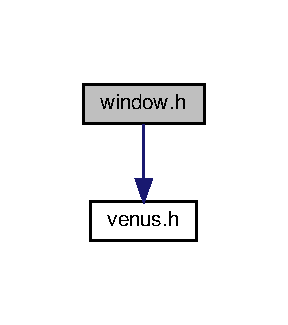
\includegraphics[width=240pt]{window_8h__incl}
\end{center}
\end{figure}
This graph shows which files directly or indirectly include this file\+:\nopagebreak
\begin{figure}[H]
\begin{center}
\leavevmode
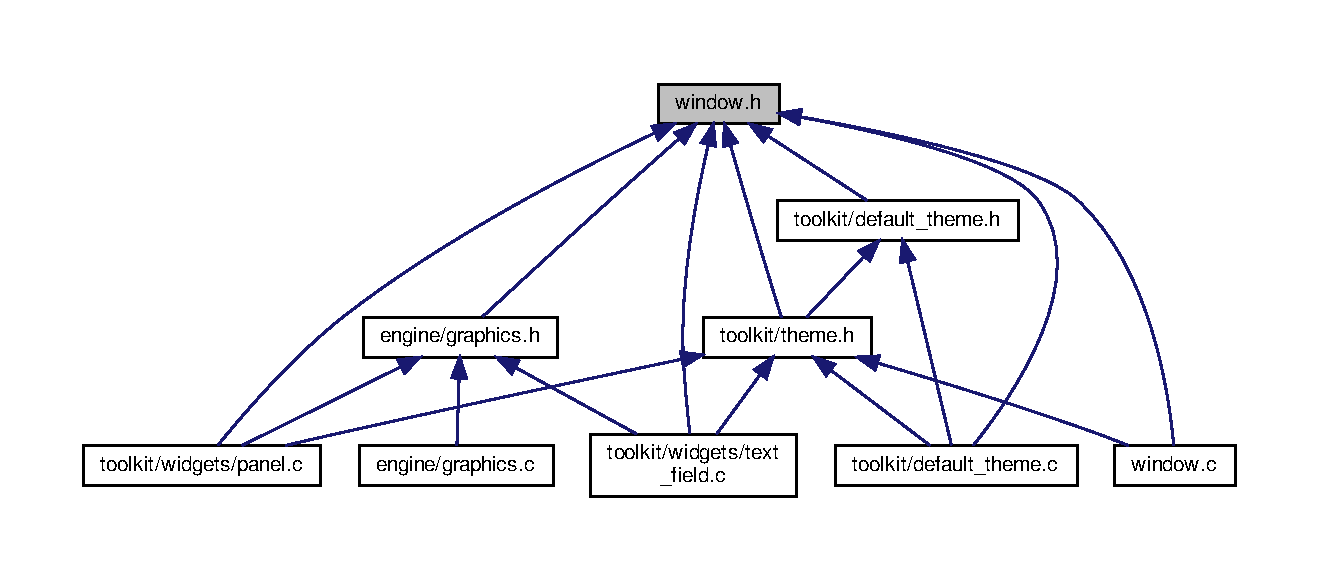
\includegraphics[width=350pt]{window_8h__dep__incl}
\end{center}
\end{figure}
\subsection*{Data Structures}
\begin{DoxyCompactItemize}
\item 
struct \hyperlink{structwindow}{window}
\begin{DoxyCompactList}\small\item\em Structure that contains the basic building blocks for each venus window. \end{DoxyCompactList}\end{DoxyCompactItemize}
\subsection*{Typedefs}
\begin{DoxyCompactItemize}
\item 
\mbox{\Hypertarget{window_8h_afe5948374b6e875142eef3c4cd43569f}\label{window_8h_afe5948374b6e875142eef3c4cd43569f}} 
typedef unsigned long {\bfseries \+\_\+\+\_\+x\+\_\+win}
\item 
\mbox{\Hypertarget{window_8h_a4fef5df112e388e88499df7a27775168}\label{window_8h_a4fef5df112e388e88499df7a27775168}} 
typedef struct \+\_\+\+\_\+\+G\+L\+Xcontext\+Rec $\ast$ {\bfseries \+\_\+\+\_\+glx\+\_\+context}
\end{DoxyCompactItemize}
\subsection*{Functions}
\begin{DoxyCompactItemize}
\item 
int \hyperlink{window_8h_affebef5e6a51b1546cadf37adf74297a}{venus\+\_\+initialize} ()
\begin{DoxyCompactList}\small\item\em Initializes venus and the libraries used. \end{DoxyCompactList}\item 
int \hyperlink{window_8h_a7ddd3c1fff91f413837be14742e82c5e}{venus\+\_\+terminate} ()
\begin{DoxyCompactList}\small\item\em Terminates venus and does memory clean up. \end{DoxyCompactList}\item 
int \hyperlink{window_8h_aa1667db02fb07f04dfb4b96ddec6893d}{create\+\_\+window} (\hyperlink{structwindow}{window} $\ast$win)
\begin{DoxyCompactList}\small\item\em Creates a new window. \end{DoxyCompactList}\item 
int \hyperlink{window_8h_aa2ee2c8b10e2e4536bb4151990f48ac2}{destroy\+\_\+window} (\hyperlink{structwindow}{window} $\ast$win)
\begin{DoxyCompactList}\small\item\em Destroys a window. \end{DoxyCompactList}\item 
int \hyperlink{window_8h_aba54f1b4e0762bd4cc0434d4f17a87c4}{set\+\_\+title} (\hyperlink{structwindow}{window} $\ast$win, char $\ast$title)
\begin{DoxyCompactList}\small\item\em Sets a window\textquotesingle{}s title. \end{DoxyCompactList}\item 
int \hyperlink{window_8h_a25032ce093a2111eef67bdebeb5f887c}{set\+\_\+background\+\_\+color} (\hyperlink{structwindow}{window} $\ast$win, color color)
\begin{DoxyCompactList}\small\item\em Sets a window\textquotesingle{}s color. \end{DoxyCompactList}\item 
int \hyperlink{window_8h_a294b947aff88bc133591bc02f3269d51}{show} (\hyperlink{structwindow}{window} $\ast$win)
\begin{DoxyCompactList}\small\item\em Shows a window. \end{DoxyCompactList}\item 
int \hyperlink{window_8h_a1739057d6d8077a7490b0467ea5d064b}{hide} (\hyperlink{structwindow}{window} $\ast$win)
\begin{DoxyCompactList}\small\item\em Hides a window. \end{DoxyCompactList}\item 
int \hyperlink{window_8h_a6a97127a0760a0ca431456fd3fd5c087}{flush} ()
\begin{DoxyCompactList}\small\item\em Flushes all X requests. \end{DoxyCompactList}\item 
int \hyperlink{window_8h_a43891902ce142858e0ee68ce4dff0231}{venus\+\_\+begin\+\_\+loop} ()
\begin{DoxyCompactList}\small\item\em Starts the event loop for any associated venus windows. \end{DoxyCompactList}\item 
int \hyperlink{window_8h_a7d2e831da7d3e6cfd60ff95835f1c9fa}{swap\+\_\+buffers} (\hyperlink{structwindow}{window} $\ast$win)
\begin{DoxyCompactList}\small\item\em Swaps the framebuffers and clears the draw buffer. \end{DoxyCompactList}\end{DoxyCompactItemize}


\subsection{Detailed Description}
Venus Graphics Engine Copyright (C) 2020, Wesley Studt 

\subsection{Function Documentation}
\mbox{\Hypertarget{window_8h_aa1667db02fb07f04dfb4b96ddec6893d}\label{window_8h_aa1667db02fb07f04dfb4b96ddec6893d}} 
\index{window.\+h@{window.\+h}!create\+\_\+window@{create\+\_\+window}}
\index{create\+\_\+window@{create\+\_\+window}!window.\+h@{window.\+h}}
\subsubsection{\texorpdfstring{create\+\_\+window()}{create\_window()}}
{\footnotesize\ttfamily int create\+\_\+window (\begin{DoxyParamCaption}\item[{\hyperlink{structwindow}{window} $\ast$}]{win }\end{DoxyParamCaption})}



Creates a new window. 

This creates a new X window and binds a GL context to that window.


\begin{DoxyParams}{Parameters}
{\em win} & Pointer to window\\
\hline
\end{DoxyParams}
\begin{DoxyReturn}{Returns}
Returns whether it was successful or not 
\end{DoxyReturn}
\mbox{\Hypertarget{window_8h_aa2ee2c8b10e2e4536bb4151990f48ac2}\label{window_8h_aa2ee2c8b10e2e4536bb4151990f48ac2}} 
\index{window.\+h@{window.\+h}!destroy\+\_\+window@{destroy\+\_\+window}}
\index{destroy\+\_\+window@{destroy\+\_\+window}!window.\+h@{window.\+h}}
\subsubsection{\texorpdfstring{destroy\+\_\+window()}{destroy\_window()}}
{\footnotesize\ttfamily int destroy\+\_\+window (\begin{DoxyParamCaption}\item[{\hyperlink{structwindow}{window} $\ast$}]{win }\end{DoxyParamCaption})}



Destroys a window. 

You should always destroy any window you create in order to ensure that no memory is leaked.


\begin{DoxyParams}{Parameters}
{\em win} & Pointer to window\\
\hline
\end{DoxyParams}
Returns whether it was successful or not \mbox{\Hypertarget{window_8h_a6a97127a0760a0ca431456fd3fd5c087}\label{window_8h_a6a97127a0760a0ca431456fd3fd5c087}} 
\index{window.\+h@{window.\+h}!flush@{flush}}
\index{flush@{flush}!window.\+h@{window.\+h}}
\subsubsection{\texorpdfstring{flush()}{flush()}}
{\footnotesize\ttfamily int flush (\begin{DoxyParamCaption}{ }\end{DoxyParamCaption})}



Flushes all X requests. 

This is only used to tell X to flush the display. It will likely be removed soon because it won\textquotesingle{}t need to exist.

\begin{DoxyReturn}{Returns}
Returns whether it was successful or not 
\end{DoxyReturn}
\mbox{\Hypertarget{window_8h_a1739057d6d8077a7490b0467ea5d064b}\label{window_8h_a1739057d6d8077a7490b0467ea5d064b}} 
\index{window.\+h@{window.\+h}!hide@{hide}}
\index{hide@{hide}!window.\+h@{window.\+h}}
\subsubsection{\texorpdfstring{hide()}{hide()}}
{\footnotesize\ttfamily int hide (\begin{DoxyParamCaption}\item[{\hyperlink{structwindow}{window} $\ast$}]{win }\end{DoxyParamCaption})}



Hides a window. 

This requests X to unmap the window


\begin{DoxyParams}{Parameters}
{\em win} & Pointer to window\\
\hline
\end{DoxyParams}
\begin{DoxyReturn}{Returns}
Returns whether it was successful or not 
\end{DoxyReturn}
\mbox{\Hypertarget{window_8h_a25032ce093a2111eef67bdebeb5f887c}\label{window_8h_a25032ce093a2111eef67bdebeb5f887c}} 
\index{window.\+h@{window.\+h}!set\+\_\+background\+\_\+color@{set\+\_\+background\+\_\+color}}
\index{set\+\_\+background\+\_\+color@{set\+\_\+background\+\_\+color}!window.\+h@{window.\+h}}
\subsubsection{\texorpdfstring{set\+\_\+background\+\_\+color()}{set\_background\_color()}}
{\footnotesize\ttfamily int set\+\_\+background\+\_\+color (\begin{DoxyParamCaption}\item[{\hyperlink{structwindow}{window} $\ast$}]{win,  }\item[{color}]{color }\end{DoxyParamCaption})}



Sets a window\textquotesingle{}s color. 


\begin{DoxyParams}{Parameters}
{\em win} & Pointer to window \\
\hline
{\em color} & The window\textquotesingle{}s color. Only the first three values, the red, green, and blue values, are used.\\
\hline
\end{DoxyParams}
\begin{DoxyReturn}{Returns}
Returns whether it was successful or not 
\end{DoxyReturn}
\mbox{\Hypertarget{window_8h_aba54f1b4e0762bd4cc0434d4f17a87c4}\label{window_8h_aba54f1b4e0762bd4cc0434d4f17a87c4}} 
\index{window.\+h@{window.\+h}!set\+\_\+title@{set\+\_\+title}}
\index{set\+\_\+title@{set\+\_\+title}!window.\+h@{window.\+h}}
\subsubsection{\texorpdfstring{set\+\_\+title()}{set\_title()}}
{\footnotesize\ttfamily int set\+\_\+title (\begin{DoxyParamCaption}\item[{\hyperlink{structwindow}{window} $\ast$}]{win,  }\item[{char $\ast$}]{title }\end{DoxyParamCaption})}



Sets a window\textquotesingle{}s title. 


\begin{DoxyParams}{Parameters}
{\em win} & Pointer to window \\
\hline
{\em title} & The desired title\\
\hline
\end{DoxyParams}
\begin{DoxyReturn}{Returns}
Returns whether it was successful or not 
\end{DoxyReturn}
\mbox{\Hypertarget{window_8h_a294b947aff88bc133591bc02f3269d51}\label{window_8h_a294b947aff88bc133591bc02f3269d51}} 
\index{window.\+h@{window.\+h}!show@{show}}
\index{show@{show}!window.\+h@{window.\+h}}
\subsubsection{\texorpdfstring{show()}{show()}}
{\footnotesize\ttfamily int show (\begin{DoxyParamCaption}\item[{\hyperlink{structwindow}{window} $\ast$}]{win }\end{DoxyParamCaption})}



Shows a window. 

This requests X to map the window


\begin{DoxyParams}{Parameters}
{\em win} & Pointer to window\\
\hline
\end{DoxyParams}
\begin{DoxyReturn}{Returns}
Returns whether it was successful or not 
\end{DoxyReturn}
\mbox{\Hypertarget{window_8h_a7d2e831da7d3e6cfd60ff95835f1c9fa}\label{window_8h_a7d2e831da7d3e6cfd60ff95835f1c9fa}} 
\index{window.\+h@{window.\+h}!swap\+\_\+buffers@{swap\+\_\+buffers}}
\index{swap\+\_\+buffers@{swap\+\_\+buffers}!window.\+h@{window.\+h}}
\subsubsection{\texorpdfstring{swap\+\_\+buffers()}{swap\_buffers()}}
{\footnotesize\ttfamily int swap\+\_\+buffers (\begin{DoxyParamCaption}\item[{\hyperlink{structwindow}{window} $\ast$}]{win }\end{DoxyParamCaption})}



Swaps the framebuffers and clears the draw buffer. 

T\+O\+DO This is just a temporary function. I will delete it later because the dev does not need access to the GL buffers

\begin{DoxyReturn}{Returns}
Returns whether it was successful or not 
\end{DoxyReturn}
\mbox{\Hypertarget{window_8h_a43891902ce142858e0ee68ce4dff0231}\label{window_8h_a43891902ce142858e0ee68ce4dff0231}} 
\index{window.\+h@{window.\+h}!venus\+\_\+begin\+\_\+loop@{venus\+\_\+begin\+\_\+loop}}
\index{venus\+\_\+begin\+\_\+loop@{venus\+\_\+begin\+\_\+loop}!window.\+h@{window.\+h}}
\subsubsection{\texorpdfstring{venus\+\_\+begin\+\_\+loop()}{venus\_begin\_loop()}}
{\footnotesize\ttfamily int venus\+\_\+begin\+\_\+loop (\begin{DoxyParamCaption}{ }\end{DoxyParamCaption})}



Starts the event loop for any associated venus windows. 

\begin{DoxyReturn}{Returns}
Returns whether it was successful or not 
\end{DoxyReturn}
\mbox{\Hypertarget{window_8h_affebef5e6a51b1546cadf37adf74297a}\label{window_8h_affebef5e6a51b1546cadf37adf74297a}} 
\index{window.\+h@{window.\+h}!venus\+\_\+initialize@{venus\+\_\+initialize}}
\index{venus\+\_\+initialize@{venus\+\_\+initialize}!window.\+h@{window.\+h}}
\subsubsection{\texorpdfstring{venus\+\_\+initialize()}{venus\_initialize()}}
{\footnotesize\ttfamily int venus\+\_\+initialize (\begin{DoxyParamCaption}{ }\end{DoxyParamCaption})}



Initializes venus and the libraries used. 

This function does a couple of important things. First it initializes zlog, the logging library I have chosen to use. zlog needs to be started first in order to start logging immediately. As well as starting zlog, it also creates a connection to an X Server. It should be noted that this does not initalize Open\+GL.

\begin{DoxyReturn}{Returns}
Returns whether it was successful or not 
\end{DoxyReturn}
\mbox{\Hypertarget{window_8h_a7ddd3c1fff91f413837be14742e82c5e}\label{window_8h_a7ddd3c1fff91f413837be14742e82c5e}} 
\index{window.\+h@{window.\+h}!venus\+\_\+terminate@{venus\+\_\+terminate}}
\index{venus\+\_\+terminate@{venus\+\_\+terminate}!window.\+h@{window.\+h}}
\subsubsection{\texorpdfstring{venus\+\_\+terminate()}{venus\_terminate()}}
{\footnotesize\ttfamily int venus\+\_\+terminate (\begin{DoxyParamCaption}{ }\end{DoxyParamCaption})}



Terminates venus and does memory clean up. 

This stops any X connections, destroys GL contexts, and finally, finishes zlog.

\begin{DoxyReturn}{Returns}
Returns whether it was successful or not 
\end{DoxyReturn}

%--- End generated contents ---

% Index
\backmatter
\newpage
\phantomsection
\clearemptydoublepage
\addcontentsline{toc}{chapter}{Index}
\printindex

\end{document}
